\documentclass[12pt]{article}
 
\usepackage[margin=1in]{geometry} 
\usepackage{amsmath,amsthm,amssymb}
\usepackage{enumerate}
\usepackage{graphicx}
\usepackage{hyperref}
\usepackage{xcolor}

\usepackage{epstopdf}
\epstopdfDeclareGraphicsRule{.tif}{png}{.png}{convert #1 \OutputFile}
\AppendGraphicsExtensions{.tif}

\graphicspath{ {/home/taylor/repos/visual/img/} }
 
\newcommand{\N}{\mathbb{N}}
\newcommand{\Z}{\mathbb{Z}}
 
\newenvironment{theorem}[2][Theorem]{\begin{trivlist}
\item[\hskip \labelsep{\bfseries #1}\hskip \labelsep{\bfseries #2.}]}{\end{trivlist}}
\newenvironment{lemma}[2][Lemma]{\begin{trivlist}
\item[\hskip \labelsep{\bfseries #1}\hskip \labelsep{\bfseries #2.}]}{\end{trivlist}}
\newenvironment{exercise}[2][Exercise]{\begin{trivlist}
\item[\hskip \labelsep{\bfseries #1}\hskip \labelsep{\bfseries #2.}]}{\end{trivlist}}
\newenvironment{problem}[2][Problem]{\begin{trivlist}
\item[\hskip \labelsep{\bfseries #1}\hskip \labelsep{\bfseries #2.}]}{\end{trivlist}}
\newenvironment{question}[2][Question]{\begin{trivlist}
\item[\hskip \labelsep{\bfseries #1}\hskip \labelsep{\bfseries #2.}]}{\end{trivlist}}
\newenvironment{corollary}[2][Corollary]{\begin{trivlist}
\item[\hskip \labelsep{\bfseries #1}\hskip \labelsep{\bfseries #2.}]}{\end{trivlist}}

\definecolor{q1color}{rgb}{0.5,1,0.5}
 
\begin{document}
 
\title{Assignment 3}
\author{Taylor Foxhall\\
tfoxhal1@binghamton.edu}
 
\maketitle

\section{Color Theory}

\begin{question}[1] {6.5}
The color corresponding to the pixel at N/2 has an RGB value of approximately
(127, 255, 127). Therefore, someone would see \textcolor{q1color}{a sickly pale
  greenish color} that turns out is very hard to read.
\end{question}

\begin{question}[2] {6.16}
Identify the gray levels in the given HSI images.
\begin{enumerate}[(a)]
  \item This image is the intersection of all the primary colors. Thus, for hue
    values, we get $H(red) = 0$, $H(yellow) = 43$, $H(green) = 85$, and $H(cyan) =
    128$. Since hue ranges from 0 to 360 and we need to scale it to 0 to 255, we
    can simply calculate the angle and scale it for the rest: $H(blue) = 170$,
    $H(magenta) = 213$ and $H(white) = 0$.
  \item Since we're working with straight primary and secondary colors, the
    saturation is 0 for black or white and 255 for anything else.
  \item By the intensity formula, the primary colors have an intensity of 85,
    the secondary colors have an intensity of 170, white has an intensity of
    255, and black has an intensity of 0.
\end{enumerate}
\end{question}

\begin{question}[3] {6.20}
Describe the HSI components of the image:
\begin{enumerate}[(a)]
  \item The HSI component images would appear as follows: the hue image would be
    four squares with the red square turning black (gray-level of 0), the green
    squares would turn dark gray (gray-level of 85), and the blue square would
    turn light gray (gray-level of 170); the saturation image would be completely
    white (gray-level of 255); the intensity image would be completely gray
    (gray-level of 85).
  \item Smoothing the saturation image would have no effect on it. The image
    would be unchanged.
  \item Since the hue image isn't entirely one level, applying an averaging mask
    would make the borders between the squares blur, and you'd see a gradient
    transition between each of the squares. 
\end{enumerate}
\end{question}
 
\section{DCT Based Image Compression}

\setcounter{MaxMatrixCols}{20}
\begin{question}[1]
Simulate DCT on some data.
\begin{enumerate}[(a)]
  \item 1x8 DCT: \[
\begin{bmatrix}
 32.526 &
 -1.281&  
 -1.306&
  0.449&
 -1.414&
 -0.300&
  0.541&
  0.254\\
 0.353 & 
 4.250 &
 0.349 &
 5.046 &
 2.474 &
 8.383 &
 1.768 &
20.388

\end{bmatrix}
\]
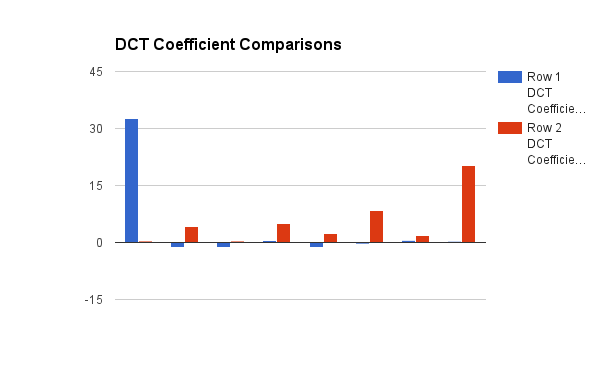
\includegraphics[scale=0.7]{dct1}\\
\item 1x16 DCT:
\[
\begin{smallmatrix}
 32.880 & 
 30.799 &
 -5.532 &
 -9.838 &
 -0.956 &
  8.537 &
 -4.596 &
 -3.632 &
  1.060 &
  4.466 &
 -8.684 &
  2.274 &
  2.309 &
  7.773 &
-20.133 &
 19.182

\end{smallmatrix}
\]
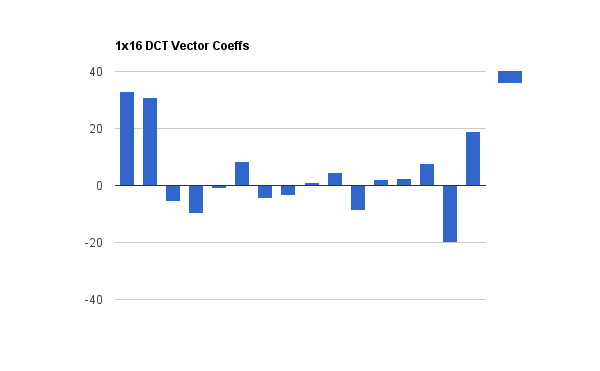
\includegraphics[scale=0.7]{dct2}\\
For this example, I think an 8-point DCT would be more useful in compression
because if we used the 16-point model, when we compress we may lose a lot of
information about the higher frequencies depending on how much we want to cut off. Say we
want to compress the image by 50\%. Then we drop the last 8 biggest frequency componenets
would be harder to reconstruct the second row. So if our image happens to
fluctuate between low and high intensities at that location, then we lose that
important information and we get a very blurry picture over a large area.
However, if we use the 8-point model, then we lose the high frequency component
information in more local areas, so we get less blurring overall.
\end{enumerate}
\end{question}

\subsection{Programming}

The algorithm behind DCT was rather simple, apply a DCT forward transform on an
image, eliminate some of its high frequency components, and restore the image
with a DCT back transform. Unfortunately the implementation fell through
somewhere.

I started with transforming the image from BGR (the way OpenCV loads it) to HSI.
The results are a bit psychedlic, but unsurprising given OpenCV still thinks
it's a BGR image.\\

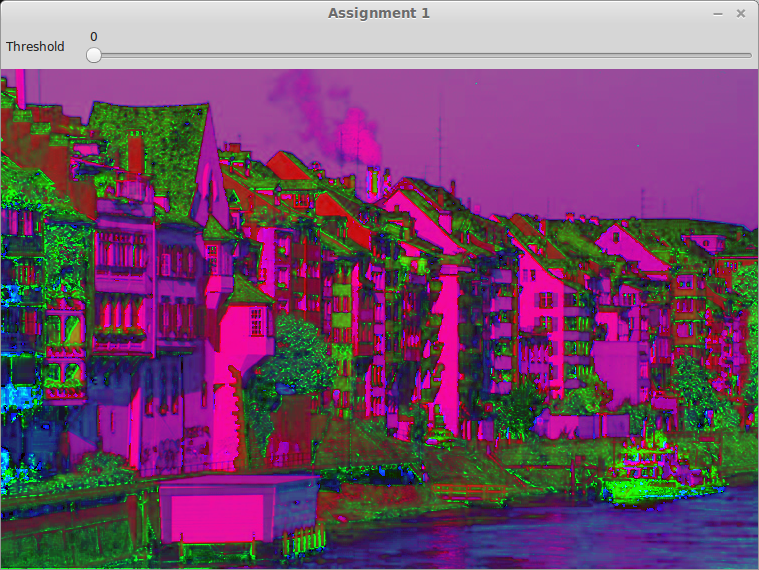
\includegraphics[scale=0.5]{baselhsi}\\

This is with hue, saturation, and intensity scaled to a range of $\lbrack0,
1\rbrack$. So, I ran it through a forward DCT transform:\\

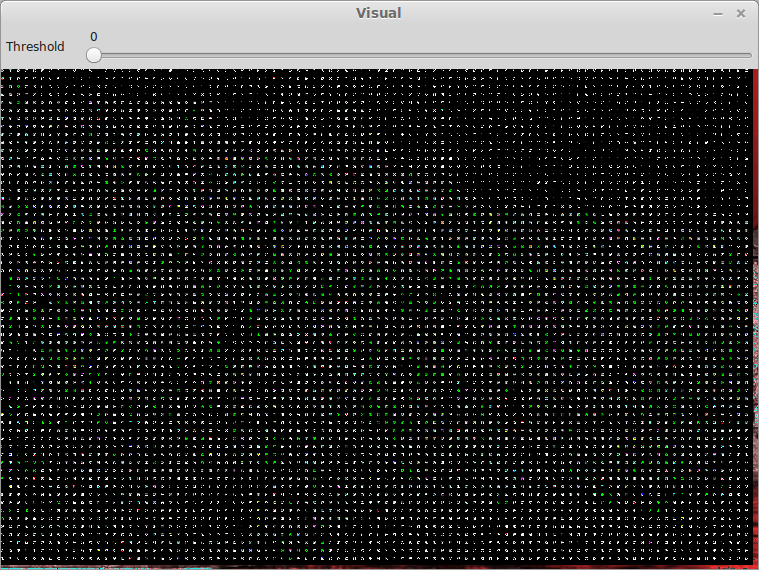
\includegraphics[scale=0.5]{baseldct3}\\

Again, this image looks odd, but it's actually unsurprising. The image itself is
fairly meaningless because all we're doing is visualizing the coefficients of
the lowest 9 frequencies of each HSI channel, placed into what OpenCV thinks is
a BGR image. But you can clearly see that for each $8\times8$ segment, we're cutting
out all but the lowest 9 frequencies. I performed a backward DCT
transform on this image:\\

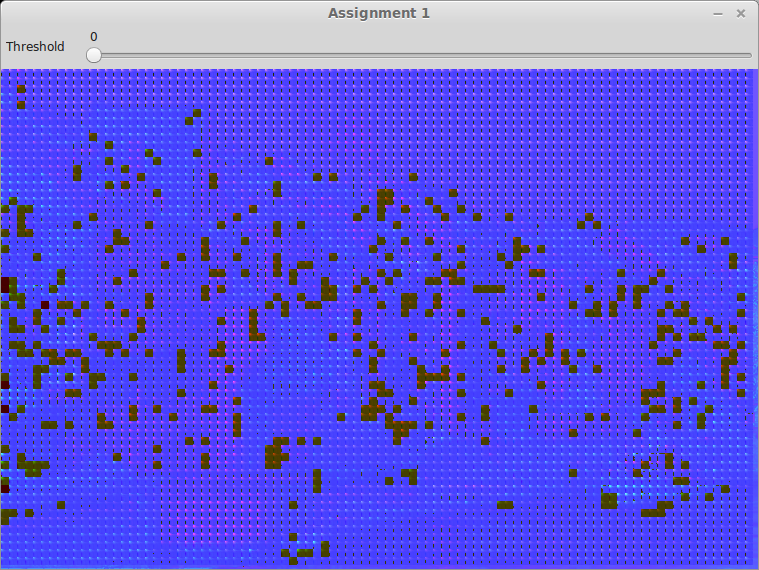
\includegraphics[scale=0.5]{baselidct3}\\

And now something looks fairly suspicious. Clearly, this is not our original
image. With the excessive amounts of purple, it also appears the hue channel has
exploded past its bound.

To try to get a better idea of what went wrong I cut out the hue and saturation channels and
inspected only the intensity channel, which basically turns it into a grayscale
image. Here's the 9-frequency forward transform:\\

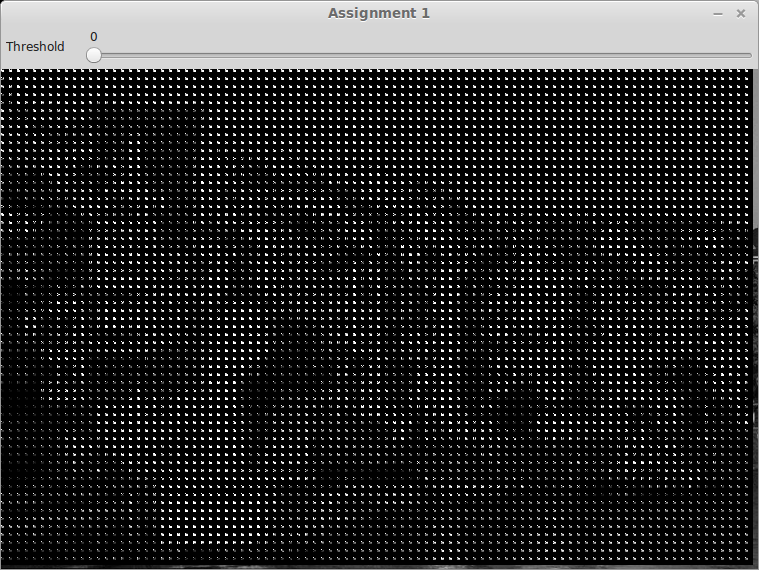
\includegraphics[scale=0.5]{baseldctg3}\\

And the corresponding inverse DCT:\\

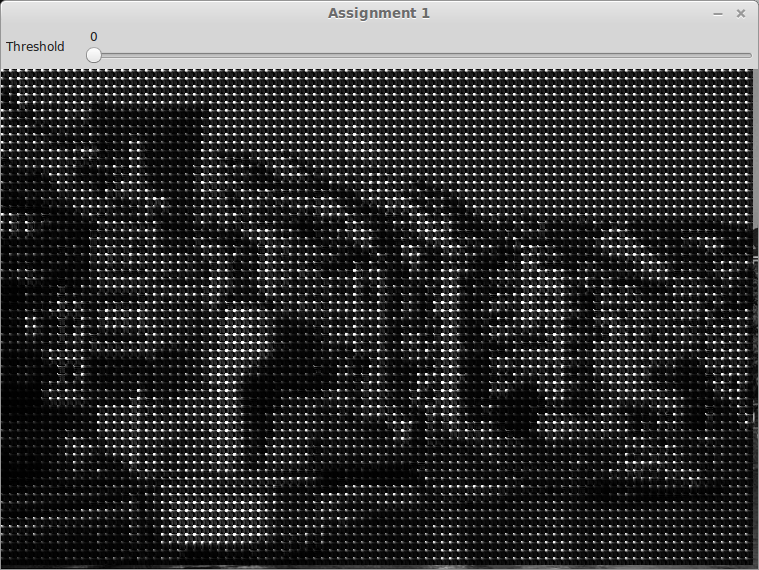
\includegraphics[scale=0.5]{baselidctg3}\\

Now we can see that it's not completely off, but the image looks like someone is
holding a wire film over it. I could not find an explanation for why this might
be.

Regardless, I ran it through DCT and IDCT again, this time only retaining the DC
frequency component:

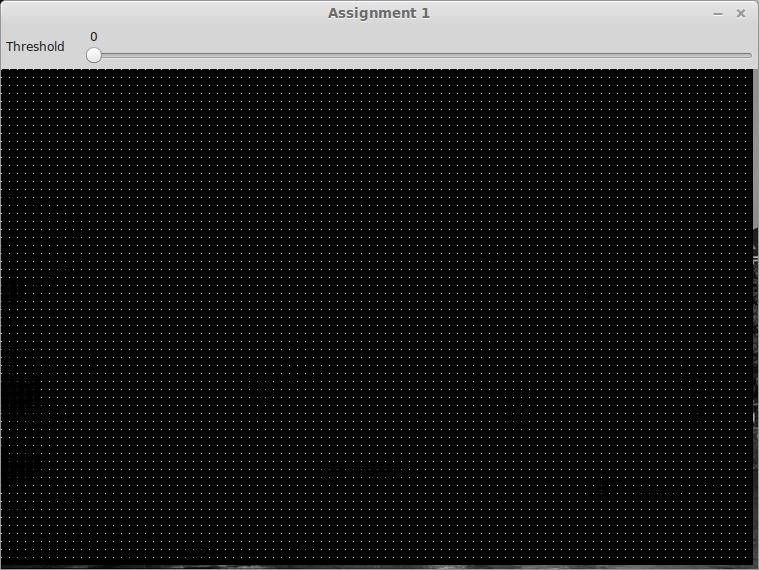
\includegraphics[scale=0.5]{baseldctg1}\\

Again, we can clearly see only one component in each $8\times8$ window is being kept,
and they don't have very much meaning when displayed as an image.\\

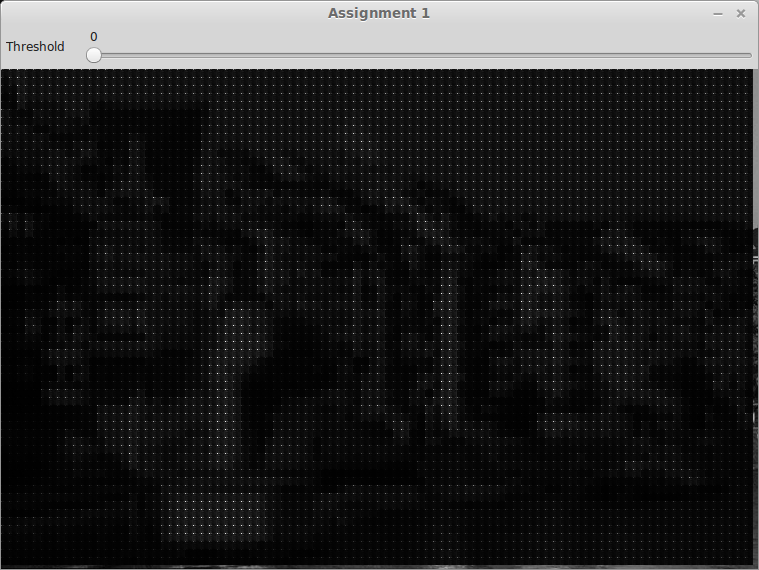
\includegraphics[scale=0.5]{baselidctg1}\\

We still get a wirey effect, but oddly enough the image seems very blurry in the
background. Out of curiosity I brightened the image by a factor of 5 to get a
bettter image. The result was interesting:\\

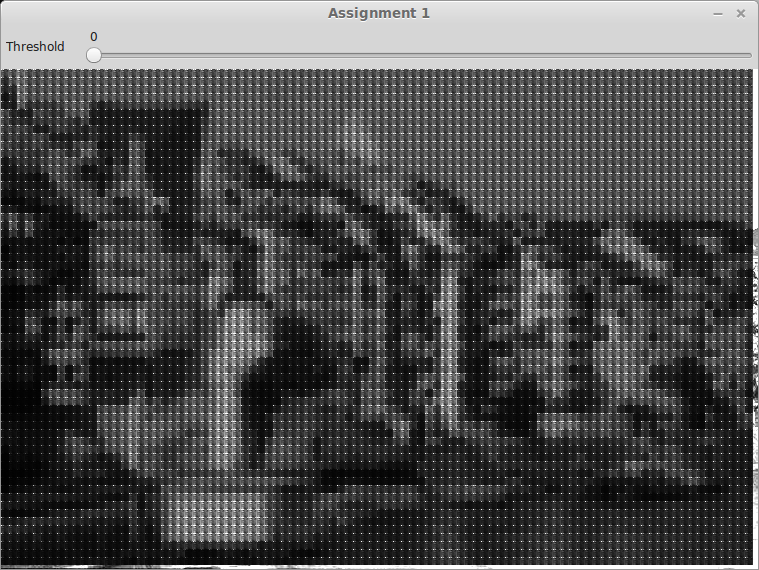
\includegraphics[scale=0.5]{baselidctg1_bright}\\

Oddly enough this image looks fairly honest to the original, despite it's
obvious low quality. Of course, I expected a lower quality than the first round
of DCT since we took out most of the frequency components. I believe this is
what the intended difference was supposed to show; R2 is supposed to be of
higher quality than R1 since it retains more of the original information.
However, I clearly am losing I'm not supposed to when I apply DCT, so it's
harder to see.

\section{ROI Segmentation}

\subsection{Linear Segments}

I implemented a linear Hough transform to detect lines in the image. Every line
can be represented as $r = x\cos{\theta} + y\sin{\theta}$ where $\theta$ is the
angle from the origin and $r$ is the distance a perpendicular line is away from
the origin at angle $\theta$. Therefore, we can transform the $xy$-plane into an
$r\theta$-plane.

Here is the image I will run a linear segmentation on:\\

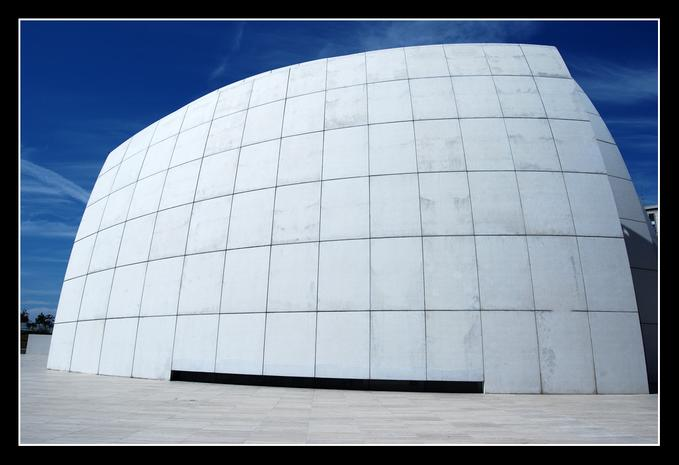
\includegraphics[scale=0.5]{Building1}\\

Before I ran the Hough transform I first had to preprocess the image a bit.
OpenCV reads in color images in BGR format, so I first converted the image to
HSI and extracted the I channel, as it was the grayscale
version of this image. Then I applied the Sobel edge detector to extract the
edges out of this image. All values above a specific hard-coded threshold were
then examined in the Hough transform. The resulting transformation is shown
below:\\

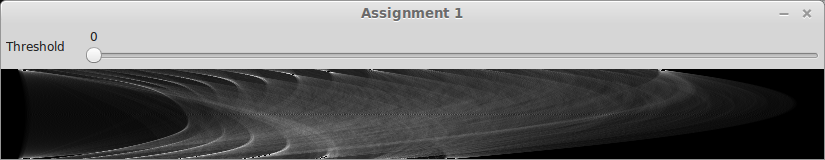
\includegraphics[height=250,width=\textwidth,trim=0 0 0 70,clip]{LinearHoughVotes}\\

This image is a little small in height because I examined values of $\theta$
from $0$ to $90$, as values from $0$ to $360$ yielded similar results. But you
can clearly see intersections of sinusodial curves, which are likely candidates
for straight lines. I took the top 50 candidates and plotted them over the
original image:

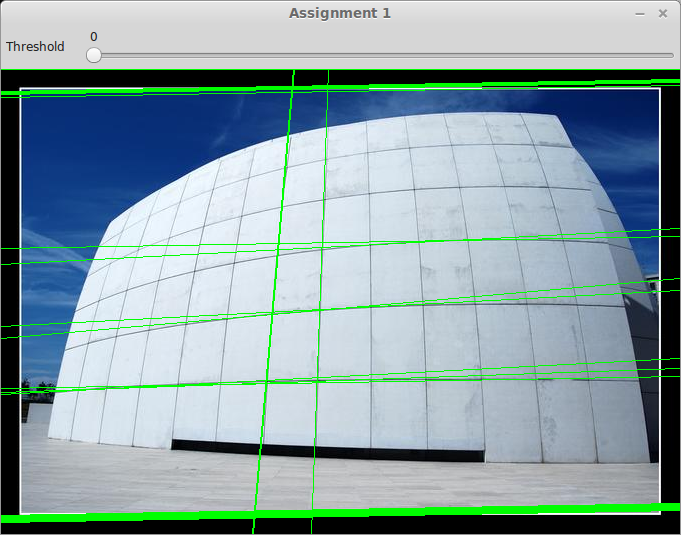
\includegraphics[scale=0.5]{Building1Hough}\\

The resulting image clearly shows the algorithm has the right idea, though it's
focusing a lot on the borders of the image, which are in fact, lines. For some
reason the segmentation seems to prefer horizontal lines as well, but this may
be specific to this image. I also hypothesize that I'd have achieved better
results had I used a Canny edge detector instead, reducing some of the extra
noise from the Sobel image.

\subsection{Circular Segments}

We can also use a Hough transform to detect circles. Similarly, since the
equation of a circle is $r^2 = {(x - x_0)}^2 + {(y - y_0)}^2$, we can transform the
$xy$-plane into $x_0y_0r$-space. This requires an extra dimension of memory, as
a result induced a serious slow down on the region detection process. However,
extrememly accurate results were achieved:\\

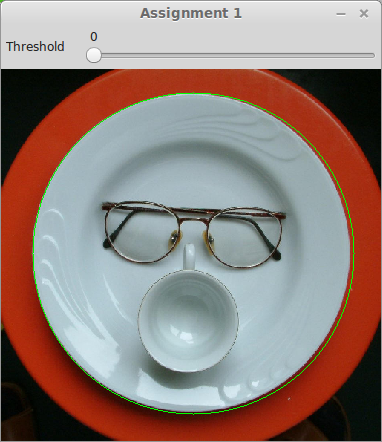
\includegraphics{DiskHough}\\

The global maxima from the entire transform yields this very clear circle around
the white plate. Admittedly, the algorithm is fairly naive. The centers could be
any valid point in the picture and the radius dimension was bounded from $0$ to
$1/2$ the image width.

Some speedup could probably be achieved by increasing the
lower bound for radii (after all, we're trying to detect big significant
circles) and possibly by changing increasing the step change of the radius. Also
for larger radii, we can gradually ignore checking the center of the
of the image. This is because the edge of a circle with a raidus larger than either half
the width or height couldn't possibly be located in the center, otherwise they'd reach
outside the border of the image. Thus, the edges of the circle must be somewhere
closer to the edges of the image. That would significantly reduce the memory
used and benefit the time as well (it takes approximately 90--120 seconds to
produce an output). Threading may also be an option for further increases in speed.

\section{References}

\begin{enumerate}
\item OpenCV 3.0 Documentation --- http://docs.opencv.org/3.0.0/
\item Hough Transforms --- https://www.youtube.com/watch?v=kMK8DjdGtZo
\item DCT --- https://www.youtube.com/watch?v={\_}bltj{\_}7Ne2c
\item Midpoint Circle Algorithm --- https://en.wikipedia.org/wiki/Midpoint{\_}circle{\_}algorithm
\end{enumerate}

\end{document}